\documentclass[a4paper,11pt,oneside,oldfontcommands]{memoir}
\usepackage{ecis2015}
\usepackage{datetime}    			% sourced from; http://ftp.snt.utwente.nl/pub/software/tex/macros/latex/contrib/datetime/
\usepackage{longtable}

%\usepackage{amssymb, setspace, rotating, titlesec, adjustbox, array, threeparttable}
\usepackage{amssymb, setspace, rotating, titlesec, adjustbox, array, threeparttable}
									% is all of this necessary?? 
%%%%%%%%%%%%%%%%%									
%% Fonts, fonts, fonts, notably for math
\usepackage{xfrac}					% tbv slanted fractions: \sfrac{}{}
\usepackage{pifont}

\RequirePackage[utf8]{inputenc}		% NOT required when using xetex as opposed to pdftex

\usepackage[T1]{fontenc}

\usepackage{amsmath}				% <amsmath> needs to be loaded before ntheorem (section 3.2.1, ftp://ftp.dante.de/pub/tex/macros/latex/contrib/ntheorem/ntheorem.pdf) 
\usepackage[mathcal]{euscript}		% tbv de gecalligrafeerde mathcal{O} en W(orld) en (M)odel etc. Refer to http://texdoc.net/texmf-dist/doc/fonts/amsfonts/euscript.pdf
									% Note that, in fact, eucal and euscript are identical, except that they use different commands (\mathcal and \mathscr). By using euscript 
									% we only provide \mathscr{} and leave \mathcal{} from amsmath unchanged
\usepackage{pgothic}				% Used for modern gothic that has a readible S
\DeclareMathAlphabet{\mathgoth}{T1}{pgoth}{m}{n}	% Declaring the pgothic family as math alphabet
%\usepackage{addfont}				% This would be an alternative for the readible S font, but not working
%\addfont[1.25]{OT1}{hge}{\hge}
%\DeclareMathAlphabet{\mathgoth}{OT1}{hge}{m}{n}	% Declaring the hge family as math alphabet

\usepackage{lmodern}				% necessary in combination with CMcal-font from mathcal/euscript to generate the font that is necessary for the Interpretation function \CMcal{I}
\usepackage{amssymb}				% necessary for (at least) the \mathbb font
\usepackage{mathrsfs}				% necessary for (at least) the \mathpzc font
\DeclareMathAlphabet{\mathpzc}{OT1}{pzc}{l}{it}		% Declaring the pzc font as math alphabet (not used, yet)


\usepackage[normalem]{ulem}			% tbv strikout text: \sout{deze tekst is strikeout}
\usepackage{siunitx}				% Necessary??

%\usepackage{fourier} 				% Assuming that you are using venturis for text, Hirwen Harendal, who designed the collection, advises that the best choice for mathematics is
									%	fourier and the second best is mathdesign. Fourier sets text and math fonts.
\usepackage{venturis2}				% Ik wil het font Venturis ADF No2 toepassen als Normalfont
									% 	Ik kan ook overwegen Obyknovennaya Novaya te gebruiken, ook fraai. Gevonden op http://www.tug.dk/FontCatalogue/venturisadfno2/

%% End of Fonts
%%%%%%%%%%%%%%%

\usepackage{xcolor}
%%\usepackage{MnSymbol}				% Levert foutmelding: Too many math alphabets used in version normal. 
\usepackage[xindy,toc]{glossaries}	%%%% The glossaries environment. Refer to: http://en.wikibooks.org/wiki/LaTeX/Glossary
%%%\usepackage{pst-plot}				%%%% The ps trick environment. Zie ook: http://tug.org/PSTricks/main.cgi?file=examples REQUIRES --latex-engine=xelatex

%% Theorems
\usepackage[ntheorem]{empheq}
\usepackage[thmmarks]{ntheorem}		% Easier handling of theorem-like environments. refer to ftp://ftp.dante.de/pub/tex/macros/latex/contrib/ntheorem/ntheorem.pdf

\usepackage{datetime}    			 % sourced from; http://ftp.snt.utwente.nl/pub/software/tex/macros/latex/contrib/datetime/
\usepackage{mdframed}

%% Figures and table placement		% Sourced from http://tug.ctan.org/tex-archive/info/epslatex/english/epslatex.pdf page 55
\usepackage{flafter}				% Ensure that the figures/tables appear after its figure/table environment definition in the text

\makeatletter						% Change the default figure / table placement from [tbp] to [htbp]; this is useful since mmd prevents us to insert the placement parameters ourselves
\def\fps@figure{htbp}
\def\fps@table{htbp}
\makeatother

\usepackage[section]{placeins}		% Since it is often desirable to keep floats in the section in which they were issued, insert a \FloatBarrier command before each section.

%% Drawings by LaTeXDraw
%\usepackage{auto-pst-pdf}			% To use pstricks in pdflatex: https://tex.stackexchange.com/questions/8413/how-to-use-pstricks-in-pdflatex
%\usepackage[pdf,usenames,dvipsnames]{pstricks}
%\usepackage{epsfig}
%\usepackage{pst-grad} % For gradients
% \usepackage{pst-plot} % For axes
%\usepackage[space]{grffile} % For spaces in paths
%\usepackage{etoolbox} % For spaces in paths
%\makeatletter % For spaces in paths
%\patchcmd\Gread@eps{\@inputcheck#1 }{\@inputcheck"#1"\relax}{}{}
%\makeatother


%% Logical proofs
\usepackage{lplfitch}				% sourced from https://github.com/rzach/lplfitch
%									% documentation from http://ftp.snt.utwente.nl/pub/software/tex/macros/latex/contrib/lplfitch/lplfitch.pdf
%\usepackage{fitch}					% The fitch package is more simple to use than lplfitch

%% Lists
%\usepackage[ampersand]{easylist}	% The easylist environment
\usepackage{enumitem}				% List manipulation package

%% Grammars
\usepackage[epsilon]{backnaur}		% For creation of BNF grammars. Refer to http://ctan.cs.uu.nl/macros/latex/contrib/backnaur/backnaur.pdf 

%% Lorem ipsum generated text
\usepackage{blindtext}

%% ToDo's							% Creating proper todo bubbles adjacent to text. Refer to http://ctan.triasinformatica.nl/macros/latex/contrib/todonotes/todonotes.pdf
\usepackage[textsize=tiny,colorinlistoftodos]{todonotes}	

%% Cross-referencing				% Allow the format of cross-references to be determined automatically according to the “type” of cross-reference (equation, section, etc.) and the context in which the cross-reference is used.
%\usepackage{varioref}				% sourced from http://texdoc.net/texmf-dist/doc/latex/tools/varioref.pdf
\usepackage{hyperref}				% If we want to use hyperref, sometime in the future for some reason, it should be defined in between of varioref and cleveref
\usepackage{cleveref}				% sourced from http://tug.ctan.org/macros/latex/contrib/cleveref/cleveref.pdf Makes varioref clever, and reuses its work to improve its own workings. 
									% The cleveref package must be loaded after all other packages that don’t specifically support it.
									% Therefore, to be safe, we declare it as last in the document's preamble.
									% Also note that all \newtheorem definitions must be placed after the cleveref package is loaded.

%% Table stuff						% sourced from: https://tex.stackexchange.com/questions/33510/how-do-i-create-the-headings-for-this-multirow-multicolum-table
\usepackage{graphicx}
\usepackage{multirow}
\usepackage{booktabs}

%%% About this LaTeX template: %%%%%%%%%%%%%%%%%%%%%%%%%%%%%%%%%%%%%%%%%%%%%%%
%
% This template should work with any (reasonably recent) full
% installation of TeXLive or MikTeX. The "ecis2015" package loads a
% number of other packages, so if some package is missing, please
% install it using the package manager of your TeX distribution. In
% particular, if the "tikz" package is missing, you may have to install
% "pgf" or simply remove our example graphics (see figure example
% below).
%
% The file "ecis2015.sty" should be placed somewhere in your TeX Path
% (or simply in the same folder as your document).
%
% Please use PDFLaTeX to compile your document.
%
% You need not escape special characters or Umlauts like é ä ö ü ß (in 
% fact, you shouldn't), as this source is inputenc'd in UTF-8.
%
% Note for BibTeX users: We use BibLaTeX for formatting, so we use Biber
% as a sorting backend (default). 
% If you still need to use the old BibTeX program, please change the 
% BibLaTeX backend in the package file ("ecis2015.sty").
%
%%%%%%%%%%%%%%%%%%%%%%%%%%%%%%%%%%%%%%%%%%%%%%%%%%%%%%%%%%%%%%%%%%%%%%%%%%%%%%


%%% ------- mijn configs: --------- %%%
%
%% test stuff

% Redefining the paragraph level into a case - see https://tex.stackexchange.com/questions/129208/numbering-paragraphs-in-latex
\newcounter{para}
\renewcommand\paragraph[1]{%
  {\par\refstepcounter{para}\textbf{Case \thepara:\space#1\space}\label{#1}}
}

%% end test stuff


%%
%% Defining new theorem and -styles
% Its documentation can be found at ftp://ftp.dante.de/pub/tex/macros/latex/contrib/ntheorem/ntheorem.pdf
%\RequirePackage[thref, thmmarks, amsmath]{ntheorem}		% Use new theorems package as opposed to amsth, include <amsmath>-emulation by including it as an option

% Allow to repeat a theorem number to, e.g., continue with a theorem such as an example, or to add something to an existing theorem
% THIS UNFORTUNATELY DOES NOT WORK, producing a <Undefined control sequence \n <argument> \rep@title \n l.38 \newtheorem*{rep@theorem}{\rep@title}>-error
%\makeatletter
%\newtheorem*{rep@theorem}{\rep@title}
%\newcommand{\newreptheorem}[2]{%
%\newenvironment{rep#1}[1]{%
% \def\rep@title{#2 \ref{##1}}%
% \begin{rep@theorem}}%
% {\end{rep@theorem}}}
%\makeatother
	
%%%%% Theorems Definitions %%%%%%
\theoremstyle{definition}
\theoremstyle{break}		% The header for all theorems are followed by a newline
% Examples 					-- are numbered by chapter, and carry an asterisk as closing symbol
\theoremsymbol{\ensuremath{_\Box}}
\newtheorem{mmexmp}{Example}[chapter]
%\newreptheorem{mmexmp}{Example (cont'd)}
% Theses   					-- have continuous numbering scheme, and still close with the asterisk
\newtheorem{Thesis}{Thesis}
% Research Questions 		-- are enclosed with horizontal lines, and probably (?) close with the asterisk
\theoremprework{\hrule}
\theorempostwork{\hrule}
\newtheorem{mmthrq}{Research Question}
% Assumption				-- are numbered by chapter, and carry an asterisk as closing symbol
\newtheorem{mmasmptn}{Assumption}[chapter]
% Definitions & theorems	-- are numbered by chapter, and carry a black square as closing symbol
\theoremsymbol{\ensuremath{_\blacksquare}}
\newtheorem{mmdef}{Definition}[chapter]
\newtheorem{mmtrm}{Theorem}[chapter]
% Design Principles, proofs	-- are numbered by chapter, and carry an open diamond as closing symbol
\theoremsymbol{\ensuremath{_\diamond}}
\newtheorem{mmdp}{Design Principle}[chapter]
\newtheorem{mmprf}{Proof}[chapter]
% Remarks to tables, figures, whatever -- restart numbering at sections, no closing symbol
\theoremsymbol{}			% no symbol
\theorembodyfont{\upshape}	% no slanted or italics
\newtheorem{mmrmk}{Remark}[subsection]	% theorem counter resets every \subsection
\renewcommand{\themmrmk}{(\arabic{mmrmk})}	% Remove subsection from theorem counter representation

% Names of the theorems
\crefname{mmexmp}{Example}{Examples}
\crefname{Thesis}{Thesis}{Theses}
\crefname{mmthrq}{Research Question}{Research Questions}
\crefname{mmdef}{Definition}{Definitions}
\crefname{mmtrm}{Theorem}{Theorems}
\crefname{mmprf}{Proof}{Proofs}
\crefname{mmdp}{Design Principle}{Design Principles}
\crefname{mmasmptn}{Assumption}{Assumptions}
\crefname{mmrmk}{Remark}{Remarks}
\crefname{chapter}{Chapter}{Chapters}
\crefname{section}{Section}{Sections}
\crefname{figure}{Figure}{Figures}
\crefname{table}{Table}{Tables}
\crefname{equation}{Eq.}{Eqs.}

% Definition of List of Theorems (\listtheorems{<name>})
\theoremlisttype{opt}

%%%%%%%% End Theorems definitions

% Equations				-- are numbered by chapter
\numberwithin{equation}{chapter}
% Figures				-- are numbered by chapter
\numberwithin{figure}{chapter}

% package backnaur: modify the production operator
\renewcommand*{\bnfpo}{\textnormal{::=}}

% some more mnemonic terms 
\newcommand*\OK{\ding{51}}		% for the check-marks
\newcommand*\ntsa{\ensuremath{\varnothing}}	% no transcription allowed

% Create a typical column header, the content of which is rotated
\newcolumntype{R}[2]{%
 >{\adjustbox{angle=#1,lap=\width-(#2)}\bgroup}%
 l%
 <{\egroup}%
}
\newcommand*\rot{\multicolumn{1}{R{60}{1em}}}% no optional argument here, please!

% Create a command for words in a box. Refer to http://tex.stackexchange.com/questions/86569/creating-uniformly-sized-boxes-around-text, and 
%                                      for the colors to http://tex.stackexchange.com/questions/136742/changing-background-color-of-text-in-latex
\newcommand{\mywordbox}[1]{%
  {% open a group for a local setting
   \setlength{\fboxsep}{-2\fboxrule}% the rule will be inside the box boundary
   \hspace{1pt}\fcolorbox{gray!20}{blue!5}{\hspace{2pt}\strut\textbf{#1}\hspace{2pt}}\hspace{1pt}% print the box, with some padding at the left and right
%   \fbox{\hspace{2pt}\strut\text{#1}\hspace{2pt}}% print the box, with some padding at the left and right
%   \fbox{\hspace{2pt}\strut#1\hspace{2pt}}% print the box, with some padding at the left and right
  }% close the group
}


%%% Enter Document Info here: %%%%%%%%%%%%%%%%%%%%%%%%%%%%%%%%%%%%%%%%%%%%%%%%
%%%datetime package config %%%
\renewcommand{\dateseparator}{-}
%\renewcommand{\timeseparator}{}
\settimeformat{hhmmsstime}  

\maintitle{Consolidating semantic interoperability in software architectures} % ← Don't use UPPERCASE here, we do that automatically.
\subtitle{Access-and-play semantic interoperability in contemporary architectural
paradigms}
\shorttitle{} % ← This goes into the header.
\category{} % 

\date{\today}


\authors{% Separate authors by a "\par" or blank line.
Paul Brandt,\\
Eindhoven University of Technology; Netherlands Organization of Applied
Scientific Research TNO, Den Haag, The Netherlands, 

\par
Eric Grandry,\\
Luxembourg Institute of Science and Technology, Esch-sur-Alzette,
Luxembourg, 

\par
Twan Basten,\\
Eindhoven University of Technology, Eindhoven, The Netherlands, 

\par
}
\shortauthors{Paul Brandt -- } % ← This goes into the header. 

%%% BibTeX: %%%%%%%%%%%%%%%%%%%%%%%%%%%%%%%%%%%%%%%%%%%%%%%%%%%%%%%%%%%%%%%%%%

\addbibresource{src/bib/CitedByMe-2018\_archSIOp.bib} % ← Your .bib file, if you're using BibTeX

%%%%%%%%%%%%%%%%%%%%%%%%%%%%%%%%%%%%%%%%%%%%%%%%%%%%%%%%%%%%%%%%%%%%%%%%%%%%%%

%%% Glossaries: %%%%%%%%%%%%%%%%%%%%%%%%%%%%%%%%%%%%%%%%%%%%%%%%%%%%%%%%%%%%%%

%%%%%%%%%%%%%%%%%%%%%%%%%%%%%%%%%%%%%%%%%%%%%%%%%%%%%%%%%%%%%%%%%%%%%%%%%%%%%%

\begin{document}
% Set the properties of the easylist

%\pagebreak

% --- Abstract --- --- --- --- ---
\begin{abstract}
\emph{Background:} Access-and-Play SIOp is the next glass ceiling in
{[}interoperability/IT-based business collaboration{]}. We can think of
two approaches to break through the ceiling, i.e., using either strong
AI (a system that can \emph{think} and has a \emph{mind}, in the
philosophical definition of the term) or weak AI (a system that can only
\emph{act} like it thinks and has a mind (Searle 1980)). Strong AI is
not yet available, while weak AI, despite its current applications in
Semantic Web or ontologies, has not yet been embedded in contemporary
software architectural paradigms. Current approaches towards SIOp can be
considered accepted folklore.

\emph{Objective:} The objective of this study is to identify and define
the (weak AI based) fundamental guidance towards access-and-play
semantic interoperability in contemporary architectural paradigms.

\emph{Method:} Our approach is based on the discipline of semiotics.
After identifying semiotic shortcomings in MDA and view-based
architectural paradigms and their subsequent definition as missing
concerns, we develop the necessary guiding architectural principles. We
finally consolidate their fundamentals as an ISO-42010 Architecture
Viewpoint to disclose them for the various architectural paradigms.
{[}We evaluate these principles by designing a reference architecture
and proof its use in SIOp between two software agents.{]}

\emph{Results:} The semiotic approach/discipline demonstrates/proves
semantics in software to be the result of a reciprocity between data and
the software code that operates on them. The major shortcomings in
architectural paradigms to account for semantic interoperability are
their negligence of semiotic fundamentals and, particularly, the absence
of an explicit ontological commitment that stands at the root of
semantics. Therefore, the concern about a semantic loose coupling should
be added to the architectural paradigms. The supporting principles are
(i) semantic transparency, (ii) semantic separation of concerns, and
(iii) explicit computational semantics. In view-based architectures
their consolidation implies a new semantic view, while the MDA paradigm
requires an ontological commitment on M3. Both paradigms need to include
a semantic alignment processing mediation capability.

\emph{Conclusions:} Access-and-play SIOp can be achieved when
considering semiotic fundamentals and adding loosely coupled formal
semantics to contemporary architectural paradigms.\\
\end{abstract}


% --- Keywords --- --- --- --- ---



%\pagebreak
% --- table of contents --- --- --- --- ---
%
% add table of contents to pdf bookmarks


% add list of todo's that are outstanding for this text


% --- main matter --- --- --- --- ---

\hypertarget{introduction}{%
\chapter{Introduction}\label{introduction}}

Never before, data were so ubiquitous, and managed access to external
data was so easy. Because current ICT is unable to \emph{use} all that
same external, non-native data as access-and-play service, agility in
business collaboration is hampered in all domains. For instance,
consider the following (allegedly real) example of an interoperability
failure.

\begin{quote}
A German steel producer upgraded its industrial process robot. Since the
majority of the steel production process is dependent on time, from a
security point of view the decision was made to not rely on their own
internal clocks but to use the German \emph{Braunschweig Funkuhr} time
radio signal as source for the exact time instead. At the end of April
1993, when Germany went on summer time, the computer clock of the steel
producer went from 1:59 AM to 3:00 AM in one minute. This resulted in a
production line allowing molten ingots to cool for one hour less than
normal. When the process controller thought the cooling time had
expired, his actions splattered still-molten steel, damaging part of the
facility.\footnote{Source:
  http://catless.ncl.ac.uk/Risks/14.57.html\#subj1, accessed May 20,
  2018}
\end{quote}

In this simple example a tiny difference in the meaning of \texttt{time}
between the steel producer and the national time provider hampered
interoperability to the extend of damaging the steel facility. This tiny
difference rooted in the assumption by the steel producer that
\texttt{time} expressed a continuous scale whilst for the Braunschweig
Funkuhr, \texttt{time} denoted instant clock time for that time zone and
therefore represented a non-continuous scale. In order to achieve that
both collaborators, here the Braunschweig Funkuhr and the steel
producer, can actually \emph{use} their peers data, the need exists to
design and implement wrappers that remove any inconsistency between the
variations that may occur in terms, structures, dimensions and what have
you. Many such variations exist, leading to a range of failures in
so-called \emph{semantic interoperability} (SIOp) and Section/Appendix
\#\# provides for a short overview of SIOp-faults. Unfortunately, it is
fundamentally impossible to automate the production of wrappers, because
we need a genuine \emph{understanding} upfront, which computers still
cannot do.

The most disconcerting consequences of a lack of (automated) SIOp are
time-to-deliver, flat interoperability failures, and even seemingly
correct but quite invalid data analysis probably leading to devastating
system behaviour. Current SIOp implementations are essentially based on
the (time-consuming) process of establishing a (local) convention on the
semantics of the terms that are exchanged during collaboration,
requiring custom solutions and collaboration-dependent software
adaptations. Such conventions can be considered a semantic monolith,
which makes dealing with data outside the monolith impossible, unless
again a time consuming (months) semantic adoption process is applied.
Moreover, these semantic conventions consider semantic heterogeneity as
a bug instead of a feature necessary to achieve semantic accuracy. But
still, this conventions-based approach towards SIOp is accepted folklore
in ICT. In view of the large uptake of the Internet, the Internet of
Things (IoT), cloud computing and big data, and in view of economical
pressure to intensify enterprise collaboration, we consider this
approach ``too little, too late''.

In comparison, scalability was a big architectural concern in the past,
requiring custom solutions as well. In response to this concern,
scalability was standardised in the form of architectural patterns, and
finally totally embedded and hidden into the infrastructure. Similarly,
SIOp can be considered the architectural concern of this decade, and we
first need to provide a standardised solution pattern to address
semantic concerns, before we can embed it in a technological
infrastructure so that SIOp becomes transparent to the developer. Where
scalability resulted in a huge increase in performance-demanding
applications against a fraction of the original costs and effort,
business agility will emerge once the semantic monolith is removed and
semantic services exist at the infrastructural level. Then SIOp becomes
an access-and-play operation that achieves SIOp in due time with data
not anticipated for during software design, at any point in their life
cycle. Metaphorically speaking, we consider SIOp as a \emph{bridge}
overarching a (semantic) gap: with \emph{bridgeheads} on each side of
the gap, with a \emph{spanning} resting on them to structurally support
the bridge and its traffic, and with a \emph{roadway} enabling the
crossing of the traffic. Finally, architectural \emph{principles}
provide the necessary guidance to the architect for the various design
decisions that effectively result in a particular bridge over a
particular (semantic) gap. Our contributions to consolidating semantic
interoperability in software architectures are fivefold, and represented
as architectural principles and concerns, as follows:

\begin{itemize}
\tightlist
\item
  \emph{Principles}: We base SIOp on establishing loose-coupling at the
  semantic level by introducing principles on semantic separation of
  concerns and semantic transparency (Section \ref{siop-principles}),
  and show how these principles can be operationalised;
\item
  \emph{Semantic concerns (bridgehead)}: Abstracting semantics from a
  tacit software implication into a tangible, computational and distinct
  artifact provides us with the potential to connect to it and to make
  comparisons with the semantic artifact of the peer software agent.
  Based on the discipline of semiotics, we explain the shortcomings of
  the current approach towards software semantics that rely on
  information models and information views. Instead, we provide for a
  fundamental notion on the application of ontologies {[}and ontological
  commitment{]} to remedy current semantic shortcomings, and we show
  {[}its/their{]} proper position in the total architecture (Section
  \ref{bridgehead-semantics});
\item
  \emph{Weak AI concerns (spanning)}: Since ``strong AI'' does not yet
  exist, SIOp remains in demand of human intervention in order to
  reconcile the semantic differences between collaborating software
  agents. However, human intervention is time consuming. We reduce the
  necessary human intervention to complement weak AI to a task that
  suffices to achieve SIOp, viz. authoring semantic alignments only
  (Section \ref{spanning-alignments});
\item
  \emph{Mediation concerns (roadway)}: We provide for a prototypical
  implementation of a mediator as the necessary component to
  automatically translate data when transferred between the
  collaborating software agents (Section \ref{roadway-mediation});
\item
  \emph{ISO42010 Architecture Viewpoint}: We formulate the architectural
  consequences of the above concerns as a specific SIOp Viewpoint in
  order to consolidate SIOp for contemporary architectural paradigms
  (Section \ref{architectural-viewpoint-on-siop});
\end{itemize}

Based on these contributions we {[}argue/defend{]} that access-and-play
SIOp can be embedded and hidden in infrastructural services when
considering semiotic fundamentals and adding loosely coupled formal
semantics to contemporary architectural paradigms. To that end, we first
describe the semiotic fundamentals in
\cref{semiotics-explanation-on-semantics}.

\hypertarget{the-semiotic-and-philosophical-foundations-of-semantics}{%
\chapter{The semiotic and philosophical foundations of
semantics}\label{the-semiotic-and-philosophical-foundations-of-semantics}}

\hypertarget{semiotics}{%
\section{Semiotics}\label{semiotics}}

The discipline of semiotics is the study of signs, reality and meaning.
The meaning of a token ultimately relates to what it denotes in reality,
whilst this relation cannot be deferred from the shape, structure or
other characteristics of the token itself due to its total
arbitrariness. In the early 1900s, De Saussure used a dyadic model that
stressed that the token (the \textbf{\emph{signifier}}) and the entity
in reality (the \textbf{\emph{signified}}) were as inseparable as the
two sides of a piece of paper (Saussure 1959). This piece of paper he
called the \textbf{\emph{semiotic sign}}, denoting the whole. This
`self-containment of the sign' remains one of the major principles of
semiotics. Constructing the semiotic sign from its distinct parts is
called \textbf{\emph{semeiosis}}. The signifier, in combination with
their ability for semeiosis, provides humans with the tool to converse
with each other. The tokens provide humans with a vocabulary, the
semeiosis makes them understand about what entities they talk about.
Semantics, then, emerges as a result of the semeiosis that connects the
distinct parts of the inseparable semiotic sign.

Sanders Peirce (in: Sowa 2000) developed another model to further
investigate the semeiosis part of semantics. He built a triadic model of
the semiotic sign, including signifier and signified, and the
\emph{interpretant} which expresses the mental and, hence, individual
sense making. This triadic model of the semiotic sign was coined by
Peirce as the \emph{semiotic triangle} (ibid.), depicted in
\cref{fig:semiotic-triangles}(a), and subsequently used and modified by
Ogden and Richards (Ogden and Richards 1989), Ullman (Ullmann 1962), and
many others. We introduce our modifications, as depicted in
\cref{fig:semiotic-triangles}(b).

\begin{figure}
\hypertarget{fig:semiotic-triangles}{%
\centering
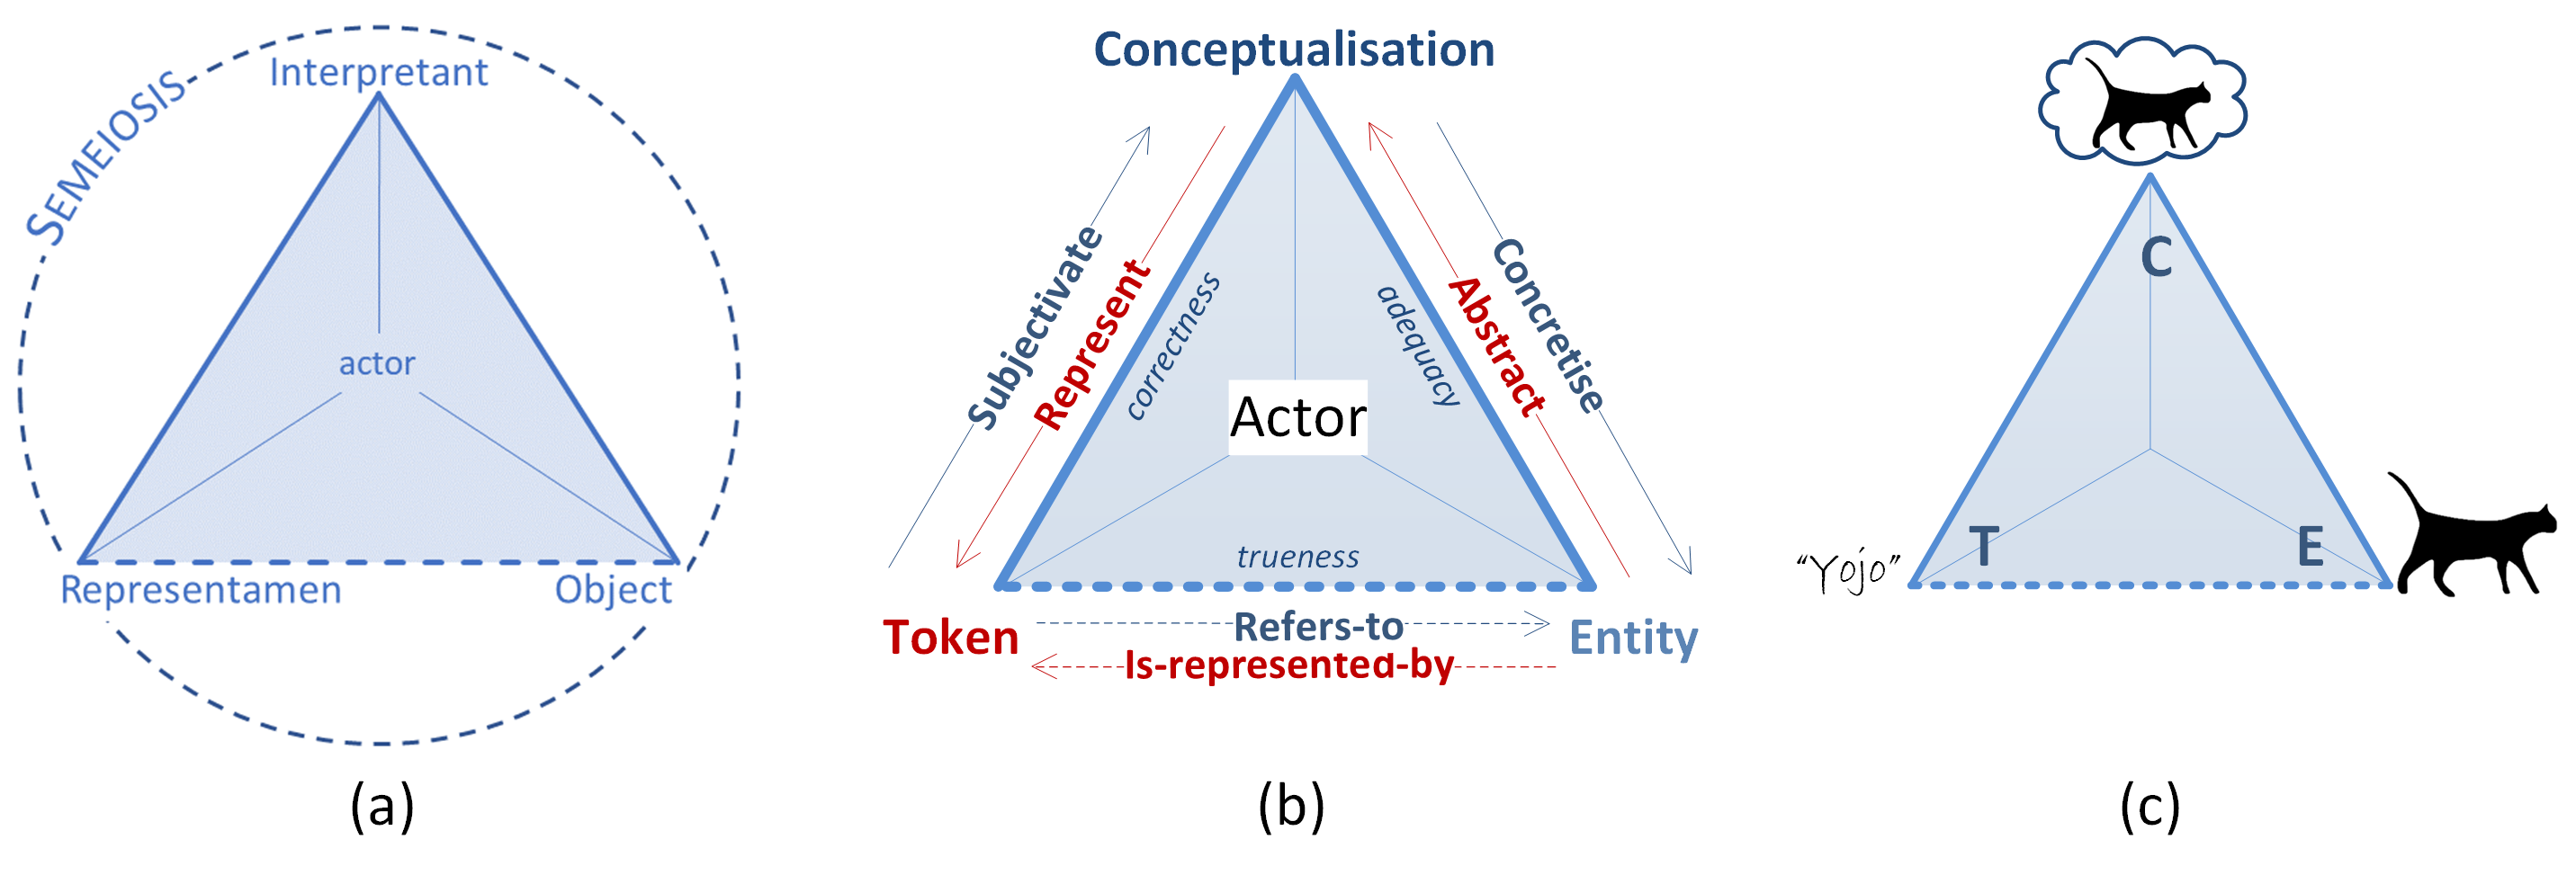
\includegraphics[width=6.25in,height=2.08333in]{src/images/SemioticTriangles.png}
\caption{The triadic model of the semiotic sign, according to Peirce
(a), and modified by us (b). Example (c) shows the concept of a cat
named ``Yojo''}\label{fig:semiotic-triangles}
}
\end{figure}

Where Peirce denotes the \emph{object}, we prefer the use of
\emph{entity} due to the ambiguous nature of the former in IT modelling
and architectures. We consider an entity to stand for a thing or an
event, but also a category of entities, a relation between entities and
a property of an entity. We will refer to the \emph{interpretant}
component as the \emph{conceptualisation}, to underline the individual
conceptualisation that is being formed during requirements analysis and
conceptual modeling. And we prefer the use of \emph{token} over
\emph{representamen}, and consider it both an atomic element as a
particular composition of atomic elements. We include denotations for
the edges that are connected to the conceptualisation vertex, and use
names that underline the individual and mental nature of the sense
making. Note that these names are directional, and must be read as the
transformations that takes place in that direction. Finally, we add the
causal characteristics that the edges represent, as introduced by (Ogden
and Richards 1989). Whenever we use ``sign'' we refer to the semiotic
sign.

\begin{figure}
\hypertarget{fig:linked-triangles}{%
\centering
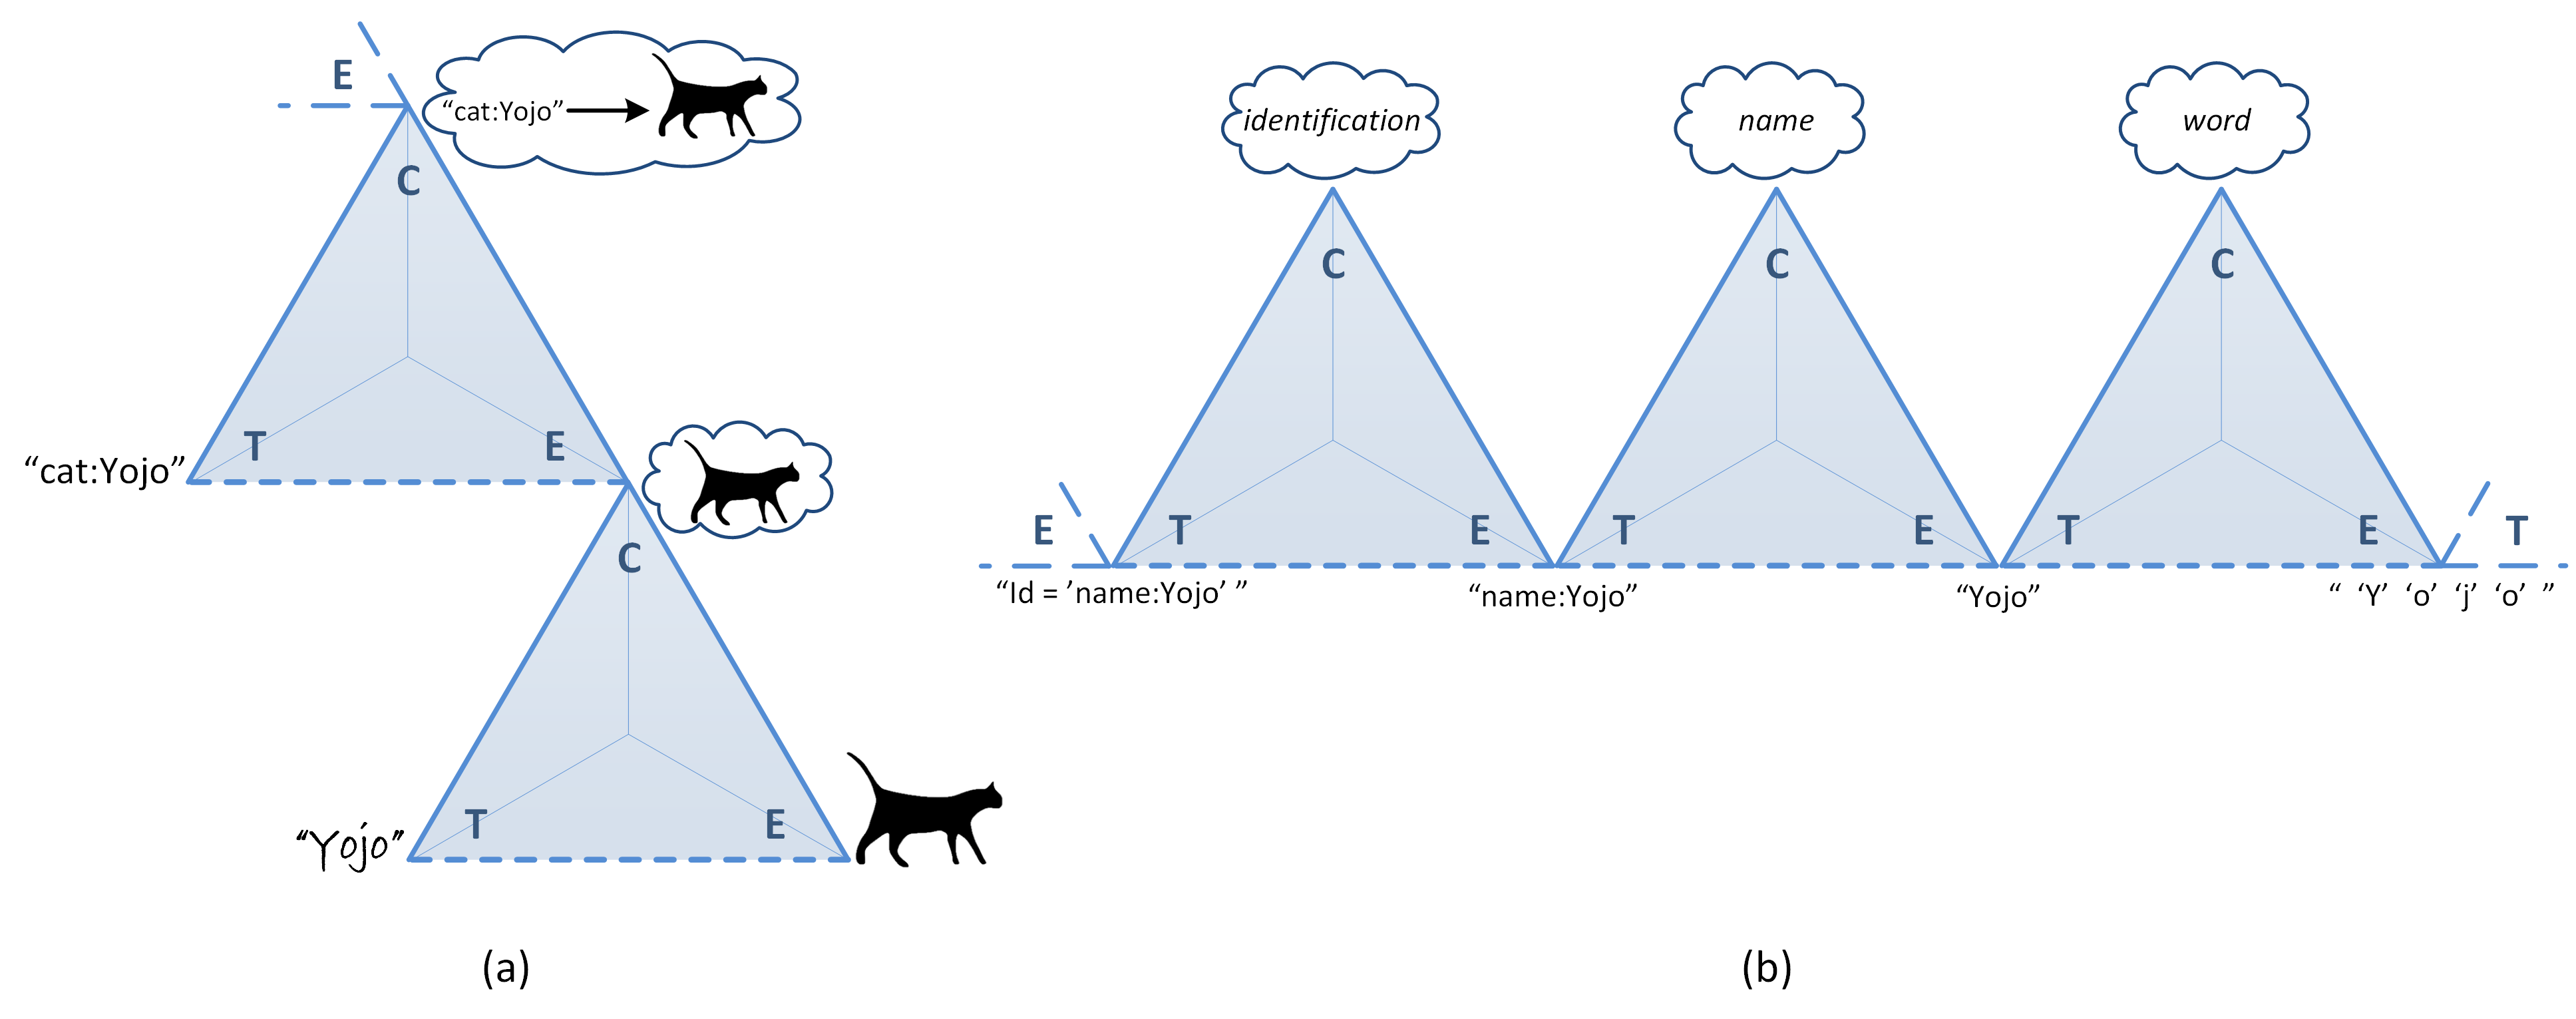
\includegraphics[width=6.25in,height=2.39583in]{src/images/LinkedTriangles.png}
\caption{Linking triadic models together.}\label{fig:linked-triangles}
}
\end{figure}

Peirce also recognised that multiple triangles could be linked together
in various ways (Sowa 2000). By stacking them together a
conceptualisation is made of ``representing an entity'': the original
concept of a \mywordbox{cat} named ``Yojo'', depicted in
\cref{fig:semiotic-triangles}(c), is being conceptualised in (a) as the
concept of a \mywordbox{cat named “Yojo”} and represented by
\mywordbox{cat:Yojo}. In (Eco 1976), Eco uses the term \emph{unlimited
semeiosis} to refer to the succession of stacking signs that emerge from
that, ad infinitum. We consider unlimited semeiosis as addressing a
dimension of comprehension about abstraction and generalisation, with an
eventual finish in the ultimate \mywordbox{Thing} concept. Linking the
triangles horizontally results in different representational metalevels,
depicted in \cref{fig:linked-triangles}(b): From right to left, the
characters ``Y'' ``o'' ``j'' and ``o'' are conceptualised as a single
\mywordbox{word} and represented as ``Yojo'', which is conceptualised as
a \mywordbox{name} and represented as ``name:Yojo'', which is
conceptualised as an \mywordbox{identifier} that might be represented as
``Id='name:Yojo'''.

\hypertarget{what-is-software-semantics}{%
\section{What is software semantics}\label{what-is-software-semantics}}

We take the position that strong AI is not yet available, if ever
(Xiuquan Li and Tao Zhang 2017), and conclude that weak AI is
essentially a token-based machine without the ability to close the gap
between token and reality. Also called the Grounding Problem (Harnad
1990), addressing this fundamental distinction in software engineering
is at best extremely narrow (Steels 2012), or not present at all (Cregan
2007). This implies that the semiotic triangle is denied its
conceptualisation vertex, and the sign remains incomplete. This leads us
to the conclusion that semantics can not ever exist in software when
based on weak AI. Unfortunately, we make do with weak AI and its
beheaded sign necessarily. This is confirmed by the software engineering
discipline herself since it consistently speaks of models that represent
reality without factoring the conceptualisation into the equation, e.g.,
``\emph{a model is a representation of reality intended for some
definite purpose}'' and similar quotes that are collected by (Aßmann et
al. 2006). Consequently, the edges that connect the conceptualisation
remain vague or necessarily conflate on the then explicit relationship
between the model and reality, depicted in
\cref{fig:software-models-reality}.

\begin{figure}
\hypertarget{fig:software-models-reality}{%
\centering
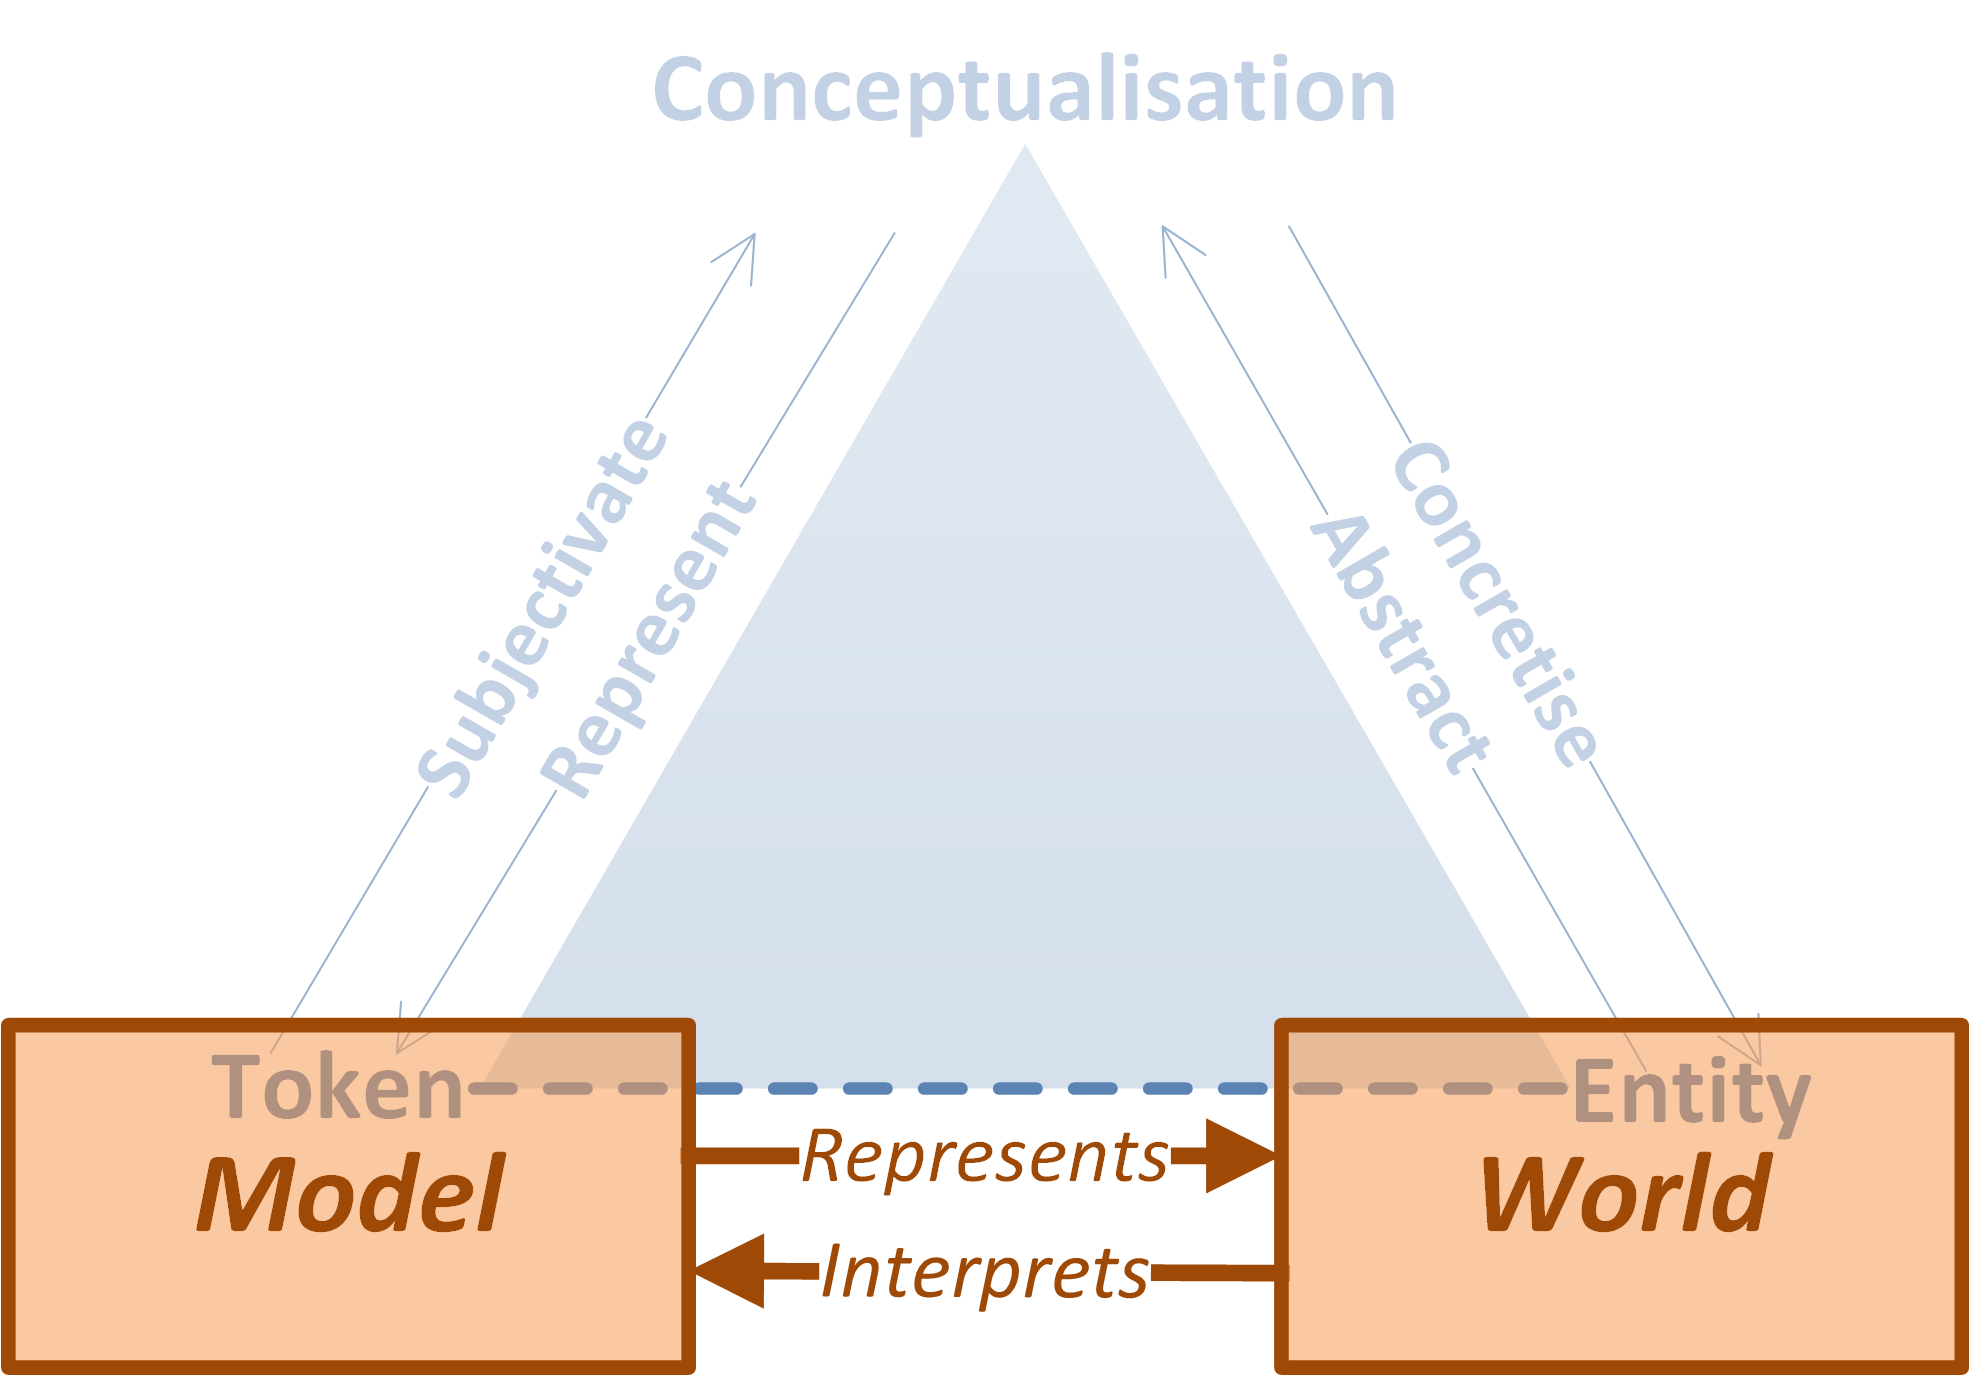
\includegraphics{src/images/SoftwareModelsReality.png}
\caption{Software engineering applies a beheaded semiotic triangle in
which its edges remain vague or conflate in the single relation between
model and reality.}\label{fig:software-models-reality}
}
\end{figure}

If we look from a semiotics perspective at the practice of software
engineering, we observe that the semeiosis is taken care of by the
software engineer whom implicitly performs the conceptualisation and
explicitly represents the conceptualisation into tokens, i.e.,
\emph{models}. The many models that software engineering typically
generate can be distinguished into those modelling the \emph{information
elements} that play a role (information or data models), and those
modelling the \emph{operations that apply} on these information elements
(process and/or business models). It is one of the responsibility of the
software engineer to keep both models in strict coherence. Eventually,
those models become code that apply on data (operations, algorithms) and
the data themselves. In case of the German steel producer, time was
represented by the information model as a continues dimension, which was
processed by the cool-down process model as a
\texttt{setWakeUpTime(currentTime\ +\ 3H)}, viz. a continues. Both
models are perfectly coherent without any reason to expect failures.
Guaranteeing this coherence is particularly important because on
run-time the software engineer has left the building, and with him the
conceptualisation vertex and the subsequent capability for semeiosis.
What remain are the model and the world that it refers to, the relation
between the two being an implicit one. The coherence between the state
of affairs in the world, viz. the data, and how this data should be
processed, is the one and only means to keep the software from failing.

In fact, the latter falls apart in two other model categories, viz.
models that directly operate on information in order to infer other
facts (conclusions), and models that act on those conclusions and
initiate some business oriented activities. We will call the latter the
\emph{pragmatics} of the software agent, and we will not further
elaborate on that. Regarding the former two models we explain them to
represent the two subtypes of meaning according to (Grice 1989; Schulz
2007): firstly, \emph{semantic} meaning, meaning as conveyed by the
tokens, explained by Grice as \emph{what is said}, are directly related
to the information models. Secondly, \emph{pragmatic} meaning, explained
by Grice as what a speaker adds by implication and/or intention when
uttering a sentence in a particular context (Smith 2003 p. 50), are
directly related to models that infer new data. For instance, consider a
heart rate reading of 128BPM. The semantic meaning that is carried is
exactly what is said, viz. the number of times a heart beats during one
minute. In case of the pragmatic meaning, though, the same bits will
refer to a very different health condition in the context of a sleeping
elderly (triggering an alarm) than in the context of a sleeping new-born
(indicating perfect health). We like to consider the pragmatic meaning
as the meaning that is required to draw conclusions, demanding the
specific \emph{context of use}.

However, as soon as the semeiosis has taken place, As we have seen in
the previous section, linking between triangles exists horizontally and
vertically alike. In this case, subsequent software engineering will
conceptualise the models in different representational metalevels as
well as built different levels of abstractions and generalisations.

the the \emph{signification} of the software agent. Although genuine
semantics does not exist in software, a software agent can definitely
fail in its signification part. When such failure happen

one of her major responsibilities are to assure that the data and the
code operating on that data remain coherent with each other. In fact,
one of the main arguments for the introduction of object-orientation
(OO) was to dispose of a means that could enforce this ``data-code
coherence'' in a natural way. Introducing a class to represent a
particular entity in reality, and its methods that operated on it,
enforces the software engineer to maintain one single conceptualisation
that is represented by a set of two tightly coupled tokens: the data and
the code operating on that data.

Interestingly, according to (Grice 1989; Schulz 2007), two subtypes of
meaning exist:

Elaborate on the reciprocity as software semantics

Elaborate on OO to consolidate the reciprocity; take the class as
example of a semantic monolith, the minimal, atomic one.

\hypertarget{ontological-commitment}{%
\section{Ontological commitment}\label{ontological-commitment}}

Apart from this strict semiotics notion, semantics are also influenced
by philosophy and need consensus on the question ``when are we committed
to the existence of certain entities?''. It is relevant to acknowledge
that humans maintain assumptions and background knowledge, both of which
impact the semeiosis and, hence, semantics. This is where the
conceptualisation plays an important role as frame of reference to our
understanding, also denoted as the \emph{ontological commitment}.
Consider the following classical sentences:

\begin{itemize}
\tightlist
\item
  Sentence 1: ``the king of France is bald''. This sentence has got a
  useful meaning, being that in case of a king of France, the dear
  fellow is as bald as a coot. We did not say \emph{that} a king of
  France exists, nor \emph{that} bald men exist; we only used these two
  phrases to \emph{refer} to things that might or might not exist.
  Hence, we do not need to commit to the existence of a king of France,
  nor to the existence of bald men, before we can formulate the sentence
  that \emph{if} there is a king of France, he must be bald. Still, and
  despite being a meaningful sentence, ``the king of France'' does not
  refer to something (as France is a republic), and therefore we cannot
  render the truth of the sentence.
\item
  Sentence 2: ``the species \emph{leo} (lions) is extinct''. Despite the
  similarity with the linguistic structure of the previous sentence, in
  this case we do need to commit to the existence of the species leo.
  The reason for this is that we do not imply here something about one
  individual but about something that many individuals have in common,
  i.e., that which defines an entity as member of the leo species.
  Without accepting that ``there is something'' that we consider
  characteristic of the species of leo and leo alone, we defy the group
  as a whole, i.e., the universal type that each of them instantiates.
  And if we defy the existence of the universal type, we defy that
  ``there is something''. But if we defy that ``there is something'', it
  would be nonsense to even speak about any of its qualities, in this
  case extinction. Therefore, by defying the existence of the species,
  we defy the meaning of the sentence itself. We therefore are forced to
  commit to the existence of the species.
\end{itemize}

The contrast exemplified by these sentences shows that only when we
commit to something (here ``the species \emph{leo}''), the theory that
we propose (here ``is extinct'') can \emph{refer} to that something in
order to \emph{establish its validity}; clearly, in our world the theory
is invalid, i.e., renders \texttt{False}, given the many counter
examples of lions being alive. We consider this the philosophical
cornerstone for semantics: we can assess the semantic validity of any
proposition if and only if the underlying ontological commitment can be
referred to. Furthermore, any assessment towards semantic
interoperability of two semantic theories cannot be made without an
assessment of the similarity between their underlying ontological
commitments. Note, however, that ``We look to (\ldots{}) Ontology not in
order to know \emph{what there is}, but in order to know what a given
remark or doctrine, ours or someone else's, \emph{says} there is''
(Quine 1961).

\hypertarget{what-is-semantic-interoperabiity}{%
\section{What is semantic
interoperabiity}\label{what-is-semantic-interoperabiity}}

\hypertarget{bridgehead-semantics}{%
\chapter{Bridgehead: Semantics}\label{bridgehead-semantics}}

\begin{enumerate}
\def\labelenumi{\arabic{enumi}.}
\tightlist
\item
  Explain shortcomings of 42010:2011 in terms of semiotic triangle:

  \begin{enumerate}
  \def\labelenumii{\arabic{enumii}.}
  \tightlist
  \item
    All models are representations of engineers' conceptualisations
  \item
    In MDA, ``models represent reality'' makes the semiotic triangle
    conflate in a \mywordbox{model}
    \textless{}---{[}\representation{]}---\textgreater{}
    \mywordbox{reality} dimension,
  \item
    This cuts-off the conceptualisation vertex and with that our
    ``knowledge about our given remark or doctrine \emph{says} there
    is''. We have removed the ``ontological level'' (Guarino 1994), and
    with that, the fact that ``terminological competence can be gained
    by formally expressing the ontological commitment of a knowledge
    base'' (ibid.)
  \item
    (Meta-)model instantiation, and hence level transition, therefore
    remains at the Term/Model vertex
  \item
    The CIM models both semantics (Domain Model) and pragmatics
    (Business Model)
  \item
    Models, including the CIM, are validated in other models, while
    ontologies are interpreted in their conceptualisation (sets and set
    theory)
  \item
    Models are ultimately expressed as either Data or Code, both located
    at the Term/Model vertex.
  \end{enumerate}
\item
  Clarify that the reciprocity between code and data manifests itself as
  software semantics

  \begin{enumerate}
  \def\labelenumii{\arabic{enumii}.}
  \tightlist
  \item
    The relationship between Data and Code is very closely coupled in
    order to maintain consistency between each other. Inconsistency
    results in software malfunction or crashes. Maintaining/controlling
    that consistency is one of the main goals of MDA/MDE.
  \item
    Inconsistency between Code and Data has either pragmatic grounds
    (i.e., code assumes different reality than data resulting in
    incorrect operations on the data) or semantic grounds (i.e., data
    assumes different reality than the code resulting in incorrect data
    being correctly operated on).
  \end{enumerate}
\end{enumerate}

An appropriate definition for ontology is given by \cite{Guarino:1998wq}
as a ``logical theory accounting for the intended meaning of a formal
vocabulary''.

The triadic model is more suitable to explain the differences between
human semantics and semantics in computers, by identifying the semiotic
differences between the two as follows. Since humans are capable of
making observations from reality, and abstract these into
conceptualisations, there is a direct connection between the entity and
the conceptualisation. Computers lack that capability, as depicted in
\cref{fig:semiotic-differences}. Here, we show the semiotic differences
between semantics as they appear for human actors, part (a) of the
Figure, and that of software actors in part (b). The comparison is made
from the perspective of communication, e.g., how is reality signified
into utterances made by the actor, and vice versa, how are utterances
signified into what they stand for in reality. We can assume the entity
to remain identical over both actors, and the token to remain equivalent
to the extent that in terms of computers these are referred to as
\emph{data}. The third node, representing the conceptualisation for
human agents, for software agents we claim to denote that as the
application. Although in its bare form an application is nothing more
than tokens that follow a specific language grammar, this bare form is
only a representation of its quintessence, i.e., a run-time notion on
how to act on the receipt of data.

However, because computers are unable to conceptualise or concretize,
the connection between the software's conceptualisation and the entity
does not exist. This ``missing link'' in artificial intelligence is
called \emph{the grounding problem}, named after the inability to ground
a conceptualisation in what it refers to in reality. In literature, two
exceptions to this rule exist, which we discuss in the box text below.
Our stance towards these exceptions is that they are interesting,
however currently irrelevant towards the resolution of semantic
interoperability due to their many practical shortcomings in
implementing an actual connection between the entity and the
conceptualisation.

\begin{figure}
\hypertarget{fig:semiotic-diffs}{%
\centering
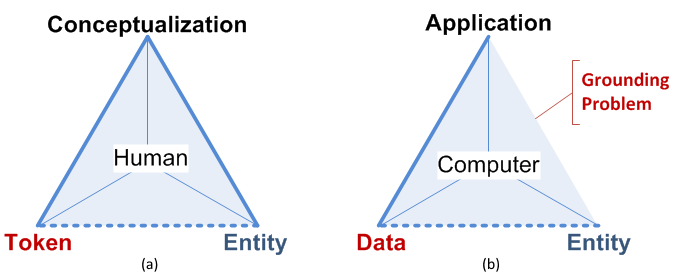
\includegraphics{src/images/SemioticDifferences.png}
\caption{Semiotic differences in semantics for humans and
computers}\label{fig:semiotic-diffs}
}
\end{figure}

This is known as the \emph{problem of reference}, a manifestation of the
\emph{grounding problem}.

In information systems, addressing the distinction between terms and
reality is extremely limited (Steels 2012), or not present at all
(Cregan 2007).

Artificial intelligence (AI) tries to tackle the grounding problem by
building some form of understanding, also known as ``strong AI''.
However, strong AI is expected to emerge on the long term only, if ever
(Xiuquan Li and Tao Zhang 2017). Its counterpart ``weak AI'',
characterised by logic and reasoning, relies on language only and can
therefore never make the step to reality on its own (Scheider 2012).

Hierin duidelijk maken wat de verschillen zijn tussen modellen en
ontologie. Semiotiek (eigenlijk de semiotische driehoek) gebruiken wij
als methode om te verklaren wat semantiek is bij mensen en bij
computers. En zonder semantiek in de architectuur, geen SIOp.

CONCLUSIE: Architectures will not be able to facilitate semantics and,
hence, consolidate SIOp without including semiotics. Assumption 1: root
cause for SIOp issues is the grounding problem: GP leads to absence of
semantics, absence of semantics leads to absence of SIOp. Fact: Strong
AI could solve GP, but doesn't exist Fact: Weak AI is based on language
only, and can never solve GP on its own Observation: Humans can solve
GP, semiotics explain why Fact: Semiotics studies relation between
language (terms) and meaning

Thus, weak AI is our only option for the time being in order to achieve
semantics and SIOp.

We therefore cannot neglect the existence of the grounding problem and
its semiotic origins. Nevertheless, we do. For instance, when we are
asked to explain how we address the grounding problem in the design of
our software agent, we can't; when we are asked to point at the
semantics parts in the code of our software agent, we can't. The same
question however about, e.g., its scalability, will render a lecture
with adequate references to the underlying architecture. We thus remain
at a loss of how to engineer semantics into software agents. However,
without a clear understanding on semantics and its contribution to the
software agent, we are lacking the bridgehead within the software agent
that is fundamental to the semantic interoperability bridge.

In fact, this is a question of philosophy while ICT is ``only'' faced
with its consequence: computers can deal with language only and have no
clue about reality.

It therefore remains impossible to ground the applied terms in reality,
denoted as the \emph{grounding problem}. Its resolution is a major
subject in strong AI and in (geographic) information science in general
\cite{Scheider:2012tj}. Although \cite{Steels:2008tr} provides for an
alternative (weak AI) solution, that only shows the need to refer to
general stance is that the grounding problem remains a big challenge .

despite the notoriously difficult philosophical questions involved,
semantic interoperability can be seen as an engineering problem, namely
that of effectively constraining interpretations towards the ones that
are considered allowable.

\hypertarget{spanning-alignments}{%
\chapter{Spanning: Alignments}\label{spanning-alignments}}

\begin{figure}
\hypertarget{fig:2semiotic-triangles}{%
\centering
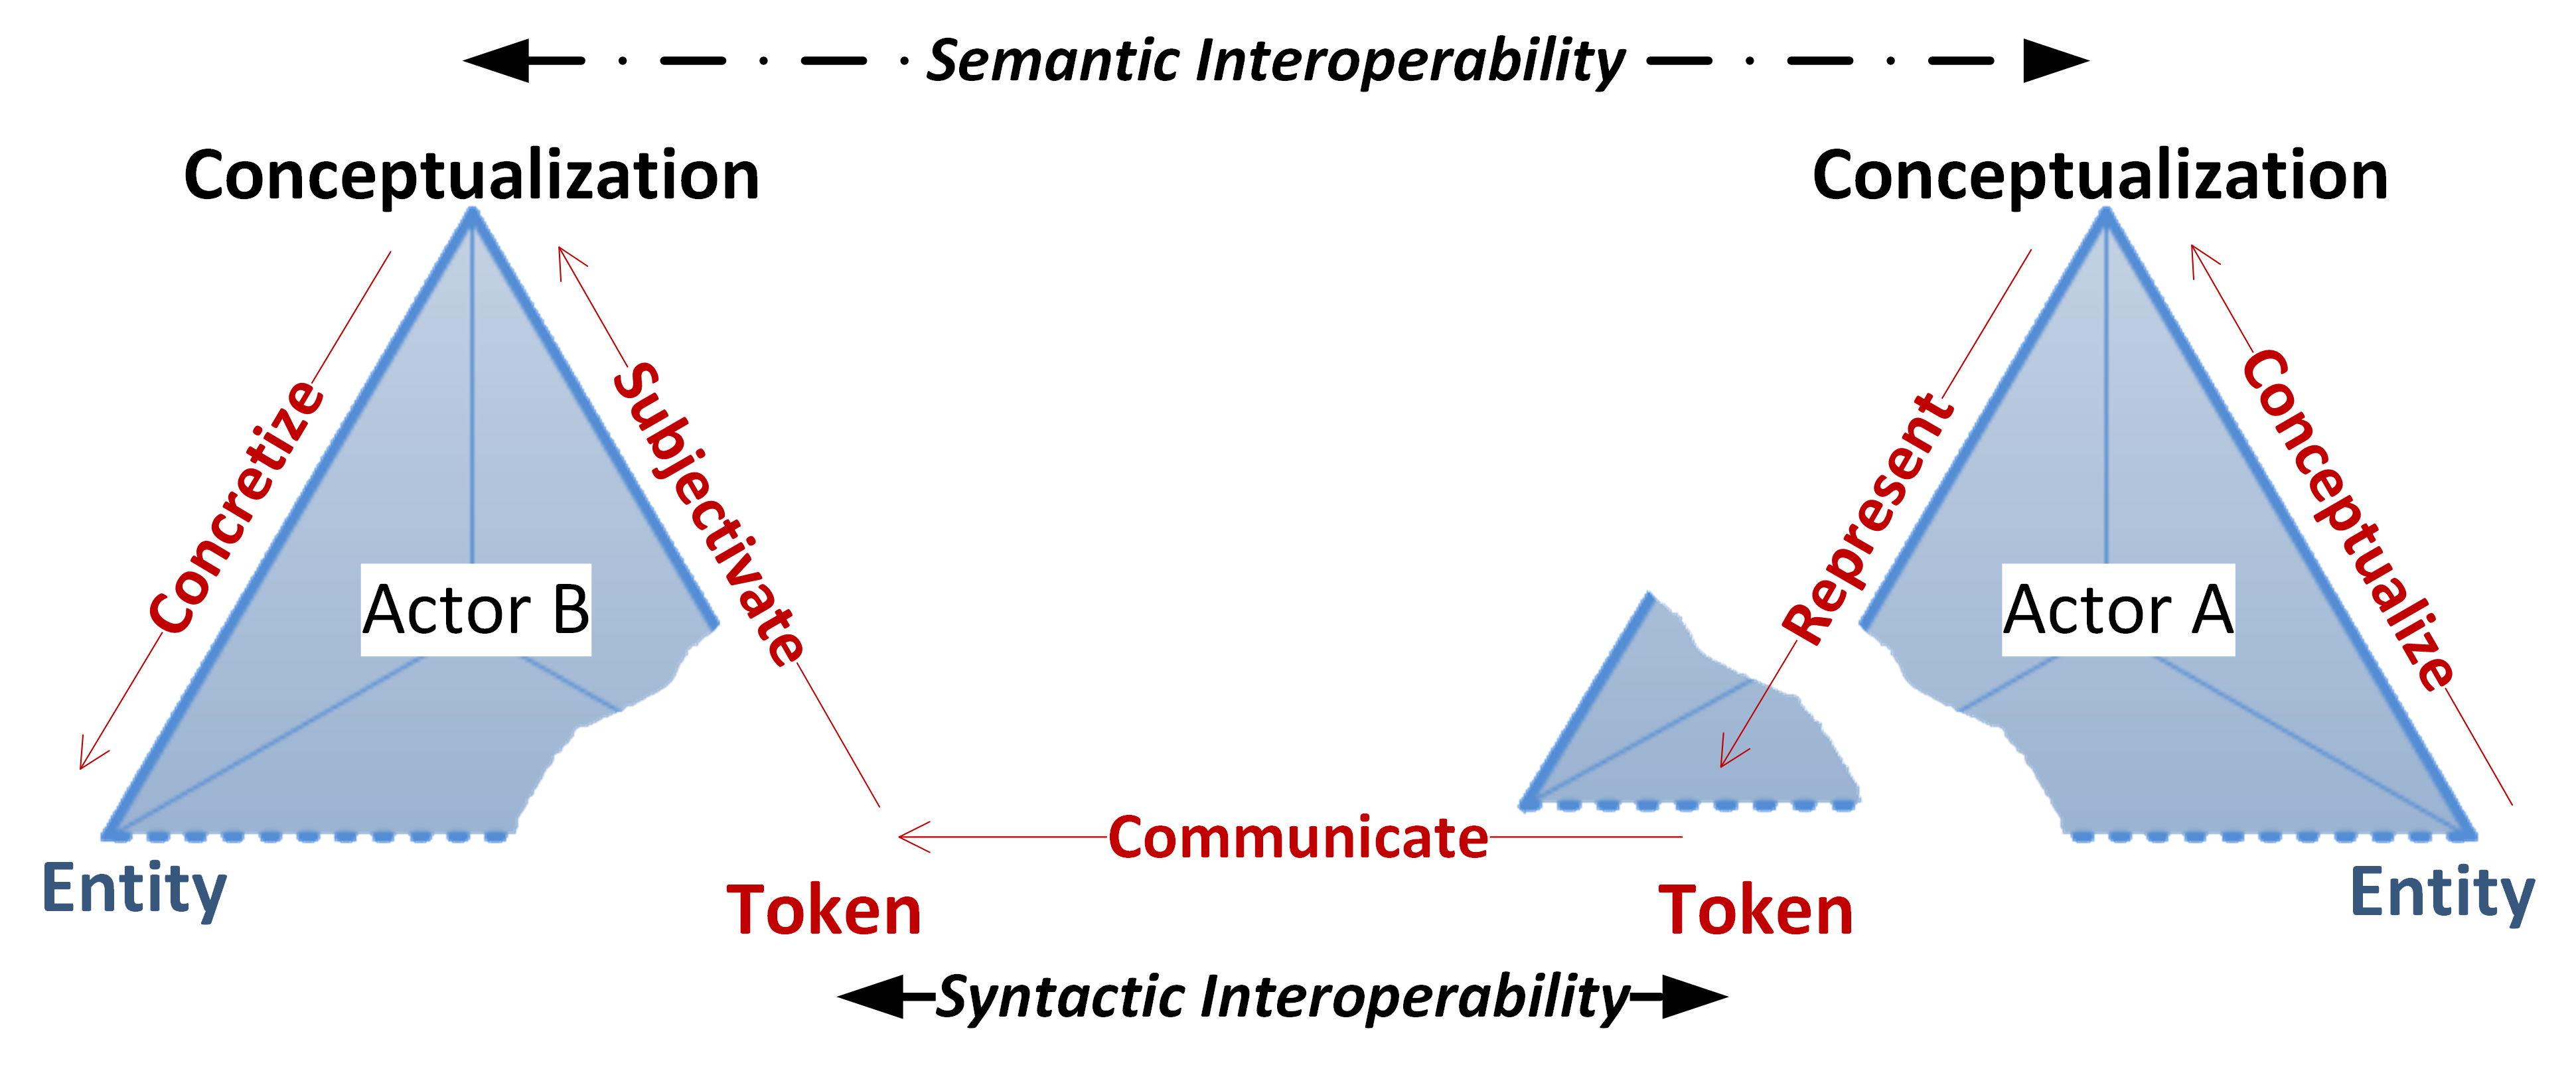
\includegraphics[width=6.25in,height=\textheight]{src/images/2SemioticTriangles.png}
\caption{The various forms of
interoperability}\label{fig:2semiotic-triangles}
}
\end{figure}

\hypertarget{roadway-mediation}{%
\chapter{Roadway: Mediation}\label{roadway-mediation}}

\hypertarget{siop-principles}{%
\chapter{SIOp Principles}\label{siop-principles}}

The main (business) requirement is to achieve SIOp as quickly as
possible, with as minimal effort as possible, for collaborations that
had not been foreseen and consequently could not be anticipated for
during design time of the (two or more) software agents.

Consequently, the software agents have been developed totally and
completely independent from each other.

This raises the following semantic concerns:

I. Loosely coupled semantics: * Define semantics once during software
design phase, and achieve SIOp many times with many different peers * EW
Dijkstra: Connected but as independent as possible: peer agents shall
only publish \emph{what} is meant with semantics, not \emph{how} it is
represented I. Scalable SIOp: * Variable in number of peers * Variable
in level of semantic heterogeneity

\begin{enumerate}
\def\labelenumi{\arabic{enumi}.}
\tightlist
\item
  Define the four semantic concerns (see \cref{fig:3Concerns} for three
  related ones):

  \begin{enumerate}
  \def\labelenumii{\roman{enumii}.}
  \tightlist
  \item
    Explicit and computational semantics by \emph{conceptual modelling}:
    Bridgehead
  \item
    Managed and controlled SIOp by \emph{semantic reconciliation}:
    Spanning
  \item
    Automated SIOp by \emph{semantic mediation}: Roadway * Address
    semantic issue about the non-equivalence between an alignment and a
    transcription (refer to (Brandt et al. 2018))
  \end{enumerate}
\end{enumerate}

\textbf{\emph{Achieve loosely coupled semantics}}

Loose coupling is founded on principles about (i) separation of
concerns, and (ii) transparency:

\begin{itemize}
\tightlist
\item
  Principle \emph{Separation of concerns}:

  \begin{itemize}
  \tightlist
  \item
    Classical:

    \begin{enumerate}
    \def\labelenumi{\roman{enumi}.}
    \tightlist
    \item
      Decompose system in parts
    \item
      with minimal functional overlap
    \end{enumerate}
  \item
    Semantical:

    \begin{enumerate}
    \def\labelenumi{\roman{enumi}.}
    \tightlist
    \item
      Separate your own semantics (i.e., conceptualisations, viz. let
      each software agent manage its own abstraction from reality)
    \item
      from establishing SIOp
    \end{enumerate}
  \end{itemize}
\item
  Principle \emph{Transparency}

  \begin{itemize}
  \tightlist
  \item
    Classical:

    \begin{enumerate}
    \def\labelenumi{\roman{enumi}.}
    \tightlist
    \item
      Agnostic to \emph{how} its functions are being achieved
    \end{enumerate}

    \begin{enumerate}
    \def\labelenumi{\arabic{enumi}.}
    \tightlist
    \item
      Communicate with minimal mutual dependency
    \end{enumerate}
  \item
    Semantical:

    \begin{enumerate}
    \def\labelenumi{\roman{enumi}.}
    \tightlist
    \item
      Agnostic to \emph{how} semantics are being achieved
    \item
      Communicate with minimal syntactic dependency, i.e., without
      agreements on semantic representation
    \end{enumerate}
  \end{itemize}
\end{itemize}

Formulate the principles in the format according to (Greefhorst and
Proper 2011)

Ad.semantic separation of concern. Where in its classical application
the result of applying the principle is that atomic functions are
defined, designed and implemented only once and remain unique, in its
semantic application the result of applying this principle is that every
software agent maintains its own semantics. Semantics are, therefore,
distributed all over the place. This seems counterintuitive or even
plain wrong, however, it is necessary for complying with the concern
about semantic scalability (in support of heterogeneous semantics).
Besides that, it is a direct consequence of the demand to allow for
independent software development

\begin{verbatim}
* Principle: specify ontological commitment as basic 
* Refer to (and partly reuse?) semantic architecture from [@Brandt2013]
\end{verbatim}

\begin{enumerate}
\def\labelenumi{\arabic{enumi}.}
\tightlist
\item
  Complement weak AI with human brain:

  \begin{itemize}
  \tightlist
  \item
    use AI where possible (computational semantics for software agent;
    supporting semantic reconciliation)
  \item
    use human brain where necessary (but not more): ontology engineering
    @ design time; alignment authoring @ pre-runtime
  \end{itemize}
\end{enumerate}

*** Achieve Scalable SIOp***

Ensure that different semantic topologies remain possible:

\begin{enumerate}
\def\labelenumi{\roman{enumi}.}
\tightlist
\item
  Star alignments (central domain ontology, aligned to local ontologies)
  for relative stable and homogeneous domain semantics

  \begin{itemize}
  \tightlist
  \item
    Good: easy semantic governance
  \item
    Bad: very similar to a semantic monolith
  \end{itemize}
\item
  Mesh alignments (bilateral alignments) for very dynamic and
  heterogeneous (domain) semantics, or low number of peers

  \begin{itemize}
  \tightlist
  \item
    Good: quickly established bilateral SIOp; granularity-on-demand,
    viz. intricate where necessary, coarse-grained where possible
  \item
    Bad: complicated semantic governance
  \end{itemize}
\item
  Mix-n-Match (coarse-grained star-alignment with specialised bilateral
  alignments) for the 70\% bulk * Good: controllable semantic
  governance; after central alignment, quickly established bilateral
  SIOp * Bad: slightly more complicated mediation due to double
  alignment support
\end{enumerate}

\begin{enumerate}
\def\labelenumi{\arabic{enumi}.}
\tightlist
\item
  Explain: difference between ontologies and models

  \begin{enumerate}
  \def\labelenumii{\roman{enumii}.}
  \tightlist
  \item
    Models lack an elaborate ontological commitment, domain ontologies
    naturally evolve on foundational ontologies (that express an
    ontological commitment)
  \item
    For prescriptive models, truth lies in themselves (deterministic
    software); ontologies are descriptive models for which the truth
    lies in reality (good for semantics)
  \item
    ontologies have open world assumption (semantic
    under-specification), models have closed world assumption (data
    remain consistent)
  \item
    Models specify systems, ontologies conceptualise entities
  \end{enumerate}

  \begin{itemize}
  \tightlist
  \item
    Try to also connect the onto/model distinction with above principles
  \item
    Induced problem: from OWA (domain ontologies) to CWA
    (information/data models)
  \item
    Principle: use domain and business ontologies for CIM (Aßmann et al.
    2006)
  \item
    Principle: prescribe requirements model with concepts that are
    defined by CIM-DO and CIM-BO (see \cref{fig:OntosInMDE}).
  \end{itemize}
\end{enumerate}

\begin{figure}
\hypertarget{fig:OntosInMDE}{%
\centering
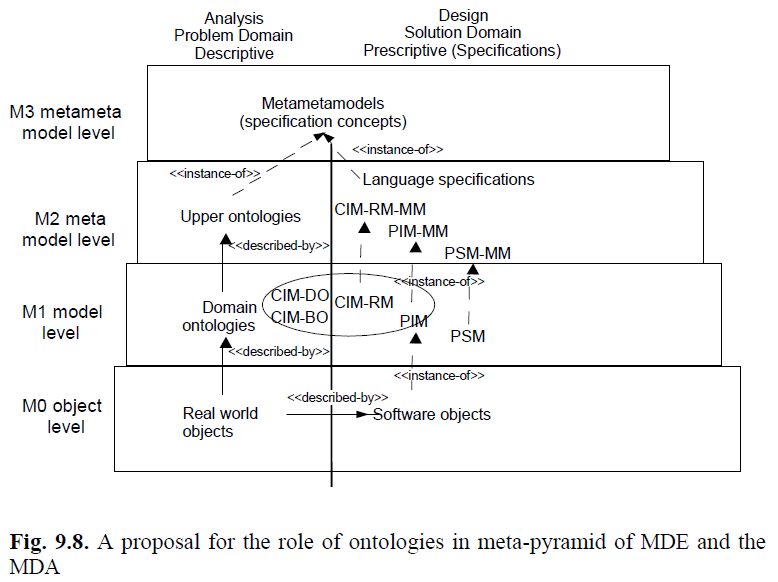
\includegraphics{src/images/OntosInMDE.png}
\caption{The use of ontologies in MDA, from (Aßmann et al.
2006)}\label{fig:OntosInMDE}
}
\end{figure}

\begin{figure}
\hypertarget{fig:3Concerns}{%
\centering
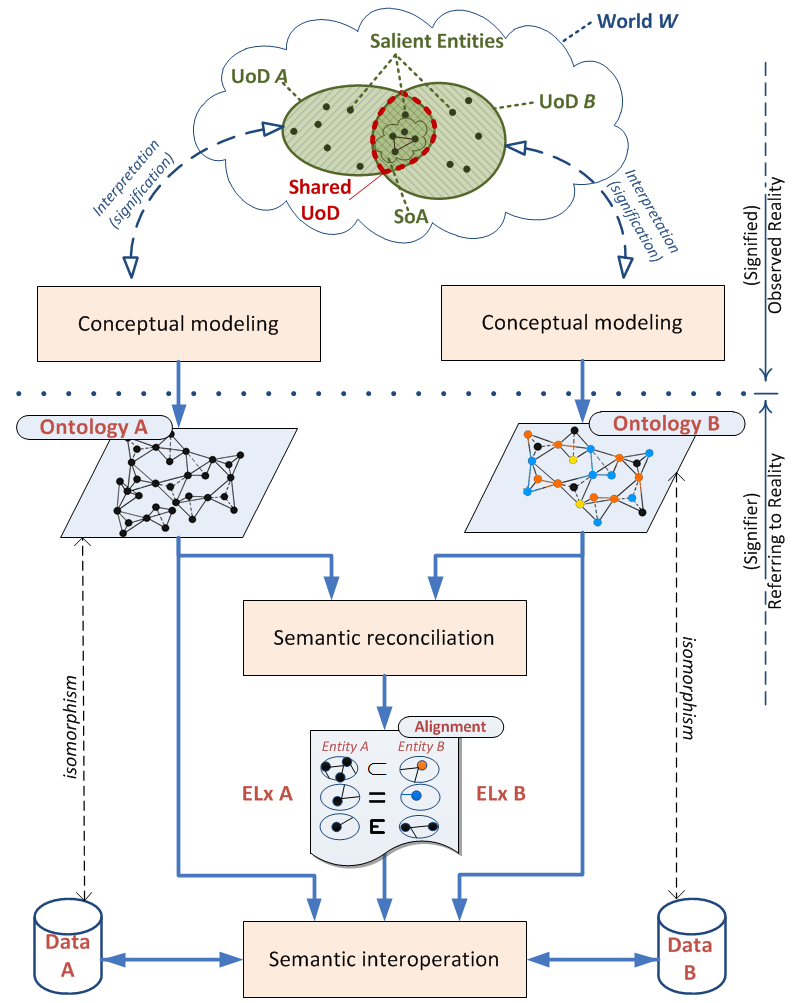
\includegraphics{src/images/3SemanticConcerns.png}
\caption{The three semantic concerns are related: conceptual modelling,
semantic reconciliation, and semantic mediation}\label{fig:3Concerns}
}
\end{figure}

\hypertarget{architectural-viewpoint-on-siop}{%
\chapter{Architectural viewpoint on
SIOp}\label{architectural-viewpoint-on-siop}}

\hypertarget{references}{%
\chapter*{References}\label{references}}
\addcontentsline{toc}{chapter}{References}

\setlength{\parindent}{-0.2in}

\setlength{\leftskip}{0.2in}

\setlength{\parskip}{8pt}

\hypertarget{refs}{}
\leavevmode\hypertarget{ref-Auxdfmann2006}{}%
Aßmann U, Zschaler S, Wagner G. 2006. Ontologies, Meta-models, and the
Model-Driven Paradigm. In \emph{Ontol. Softw. Eng. Softw. Technol.} (C.
Calero, F. Ruiz, and M. Piattinieds. ), pp. 249--273, Springer-Verlag
Berlin Heidelberg.

\leavevmode\hypertarget{ref-Brandt2018}{}%
Brandt P, Sinderen M van, Basten T. 2018. Semantic mediation: from
alignment relation to semantic identity.

\leavevmode\hypertarget{ref-Cregan2007}{}%
Cregan AM. 2007. Symbol grounding for the semantic web. W. Franconi, E
and Kifer, M and Mayed.. Semant. WEB res. Appl. Proc. 4519: 429--442.

\leavevmode\hypertarget{ref-Eco1976}{}%
Eco U. 1976. \emph{A theory of semiotics}. Indiana University Press /
London: Macmillam, Bloomington, IN.

\leavevmode\hypertarget{ref-Greefhorst2011}{}%
Greefhorst D, Proper E. 2011. \emph{Architecture Principles, The
Cornerstones of Enterprise Architecture}. Springer Berlin Heidelberg.

\leavevmode\hypertarget{ref-Grice:1991BT}{}%
Grice HP. 1989. Logic and Conversation. In \emph{Stud. W. Words}, pp.
22--40, Harvard University Press, Cambridge, MA, USA.

\leavevmode\hypertarget{ref-Guarino1994b}{}%
Guarino N. 1994. The Ontological Level. R. Casati, B. Smith, and G.
Whiteeds. Philos. Cogn. Sci. Proc. 16th int. Wittgenstein symp.
443--456;
doi:\href{https://doi.org/10.1007/978-3-642-02463-4}{10.1007/978-3-642-02463-4}.

\leavevmode\hypertarget{ref-Harnad1990}{}%
Harnad S. 1990. The Symbol Grounding Problem. Physica D 42. 335--346.

\leavevmode\hypertarget{ref-Ogden1989}{}%
Ogden CK, Richards IA. 1989. \emph{The Meaning of Meaning: A Study of
the Influence of Language upon Thought and of the Science of Symbolism}.
with a pre. Harcourt Brace Jovanovich, New York, USA.

\leavevmode\hypertarget{ref-Quine:1953er}{}%
Quine WVO. 1961. From a logical point of view. Br. Dent. J. 195: 229.

\leavevmode\hypertarget{ref-Saussure:1983ka}{}%
Saussure F de. 1959. \emph{Course in general linguistics}. C. Bally and
A. Sechehayeeds.. Philosophical Library, New York, USA.

\leavevmode\hypertarget{ref-Scheider:2012tj}{}%
Scheider S. 2012. Grounding geographic information in perceptual
operations. Dissertation, Westfälische Wilhelms-Universität Münster; IOS
Press.

\leavevmode\hypertarget{ref-Schulz2007}{}%
Schulz K. 2007. Minimal Models in Semantics and Pragmatics.
Dissertation, Universiteit van Amsterdam.

\leavevmode\hypertarget{ref-Searle:1980hw}{}%
Searle JR. 1980. Minds, brains, and programs. Behav. Brain Sci. 3:
417--424.

\leavevmode\hypertarget{ref-smith2003}{}%
Smith CS. 2003. \emph{Modes of Discourse: The Local Structure of Texts}.
Cambridge University Press, Cambridge, MA.

\leavevmode\hypertarget{ref-Sowa:2000di}{}%
Sowa JF. 2000. Ontology, metadata, and semiotics. Lect. Notes Comput.
Sci. (including Subser. Lect. Notes Artif. Intell. Lect. Notes
Bioinformatics) 1867:55--81;
doi:\href{https://doi.org/10.1007/10722280_5}{10.1007/10722280\_5}.

\leavevmode\hypertarget{ref-Steels:2008tr}{}%
Steels L. 2012. The symbol grounding problem has been solved, so what's
next. In \emph{Symb. Embodiment debates mean. Cogn.} (M. de Vega, A.
Glenberg, and A. Graessereds. ), pp. 223--244, Oxford University Press,
Oxford, UK.

\leavevmode\hypertarget{ref-Ullmann:1979sL}{}%
Ullmann S. 1962. \emph{Semantics: An Introduction to the Science of
Meaning}. 1st ed. Basil Blackwell, Oxford.

\leavevmode\hypertarget{ref-XiuquanLi2017}{}%
Xiuquan Li, Tao Zhang. 2017. An exploration on artificial intelligence
application: From security, privacy and ethic perspective. J. Zhu, E.-B.
Lin, and T. Lieds. 2017 ieee 2nd int. Conf. Cloud comput. Big data anal.
416--420;
doi:\href{https://doi.org/10.1109/ICCCBDA.2017.7951949}{10.1109/ICCCBDA.2017.7951949}.

%\chapter*{References}
% --- index --- --- --- --- ---


\printindex

%ACKNOWLEDGMENTS are optional
%\chapter*{Acknowledgments}
% % 
\end{document}
